\documentclass{article}
\usepackage[utf8]{inputenc}
\usepackage{graphicx}
\usepackage{natbib}
\usepackage{polski}
\usepackage{tabularx}
\usepackage{wrapfig}
\usepackage{enumitem}
\usepackage{multirow}
\usepackage[left=2cm,right=2cm,vmargin=2.5cm,footnotesep=0.5cm]{geometry}

\title{Historia Wrocławia}
\author{Jakub Jankowiak 258965 }
\date{Styczeń 2021}

\begin{document}
\maketitle

\tableofcontents
\clearpage
\section{Budorgium}
W czasach antycznych na obecnych terenach Wrocławia lub w bliskiej okolicy istniała miejscowość o nazwie Budorigum. Została ona odwzorowana na antycznej mapie Klaudiusza Ptolemeusza z lat 142–147 n.e.[\ref{fig: [1]}]. O tym, że miejscowość ta znajdowała się w okolicach Wrocławia, informuje Lexicon Universale [\ref{fig: [2]}] oraz wynika to z położenia wśród innych zidentyfikowanych miejscowości Śląska. Część hipotez łączy antyczną osadę Budorigum z samym Wrocławiem, część wskazuje jednak na jej lokalizację w Brzegu lub jego okolicach


\section {Założenie miasta}
Według tradycji, gród we Wrocławiu został założony przez czeskiego księcia Wratysława (cz. Vratislav I) (panował 915–921). Nazwa miasta pochodzi być może od skróconej formy imienia założyciela (Wrocisław), jednakże ekspansję na teren Śląska mógł przeprowadzić Bolesław I Srogi dopiero po roku 935, dlatego kwestia nazwy miasta jest polem do dalszych interpretacji. Według ostatnich badań nie ma śladu, który by wskazywał na funkcjonowanie wcześniej niż przed 940 rokiem grodu na wrocławskim Ostrowie Tumskim[\ref{fig: [3]}]. Nie ma więc możliwości, aby Wrocław wcześniej pełnił rolę czeskiego ośrodka administracyjnego[\ref{fig: [4]}]. W roku 985 na Ostrowie Tumskim powstał pierwszy gród wybudowany przez Mieszka I[\ref{fig: [5]}]. W tym też okresie miasto wraz z resztą Śląska przeszło we władanie rodu Piastów.

W 1000 roku na zjeździe gnieźnieńskim cesarz Otton III i Bolesław Chrobry ustanowili w mieście biskupstwo rzymskokatolickie podporządkowane arcybiskupstwu w Gnieźnie. Krótko po tym powstała w obrębie grodu pierwsza katedra romańska. Choć miasto istniało już wcześniej – datę tę traktuje się oficjalnie jako początek jego istnienia – w 2000 roku uroczyście obchodzono tysiąclecie Wrocławia. Z czasem ośrodek urbanistyczny przeniósł się na lewy brzeg Odry w okolice kościoła św. Andrzeja i Magdaleny, a potem około wieku XIII w okolice kościoła św. Elżbiety i dzisiejszego Starego Miasta.


\section {Rozwój (X–XIII wiek)}
Miasto dzieliło dzieje Śląska będąc jego centrum gospodarczym i administracyjnym. Przy osłabieniu władzy Piastów przechodziło w ręce Przemyślidów. Stało się tak m.in. w 1038, gdy w wyniku trwającego od 4 lat antychrześcijańskiego powstania doszło do najazdu czeskiego księcia Brzetysława I, a biskup wrocławski zmuszony był opuścić gród i aż do restytucji biskupstwa w 1051 rezydował najprawdopodobniej w Smogorzewie koło Namysłowa. Z okresu tego pochodzą odkryte we Wrocławiu szczątki świątyni pogańskiej z lat 30. XI wieku. Z Kroniki polskiej Galla Anonima znamy dwóch komesów Wrocławia z drugiej połowy XI w.: Magnusa i Wojsława[\ref{fig: [6]}].


W 1109 nieudane oblężenie przez króla niemieckiego Henryka V – opodal grodu na terenie dzisiejszej dzielnicy Psie Pole doszło do zwycięskiej dla Krzywoustego potyczki z armią niemiecką, zwanej bitwą na Psim Polu.

\begin{figure}[h]
	\centering
	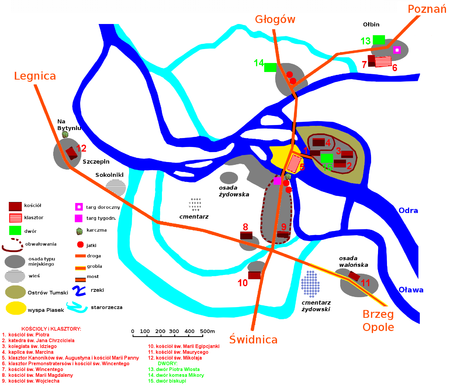
\includegraphics[scale=0.6]{Wrocław XII-XIII.png}
	\caption{Wrocław w XII-XIII}
	\label{fig: Wrocław w XII-XIII}
\end{figure}


W 1138 po podziale kraju stało się siedzibą Władysława II Wygnańca do jego wygnania przez braci. Po powrocie, z pomocą cesarską, synów księcia – Bolesława Wysokiego i Mieszka Plątonogiego, stało się siedzibą pierwszego, który objął większość ojcowizny z tytułem księcia śląskiego.

Budowa zamku książęcego na lewym brzegu Odry naprzeciw Ostrowa Tumskiego (rejon dzisiejszego Uniwersytetu Wrocławskiego) i powstające wokół niego podgrodzia zapoczątkowały przeniesienie centrum miasta w to miejsce. Współcześnie uważa się, że pierwsza lokacja miasta nastąpiła jeszcze pod rządami Henryka Brodatego, przyjmuje się daty 1214 (z tego roku zachowała się lista urzędników miejskich) lub 1226. Jednak żaden z aktów lokacyjnych miasta się nie zachował. Biorąc pod uwagę iż Wrocław był już wówczas największym miastem Śląska możliwe jest że lokacja odbyła się nawet przed 1214 rokiem. Ostrów Tumski stopniowo przechodził w posiadanie władz kościelnych. Ostatnim władcą rezydującym stale na Ostrowie był Henryk IV Probus.


Kościół św. Idziego we Wrocławiu zbudowany w latach 20 XIII wieku
W kwietniu 1241 roku wobec najazdu mongolskiego miasto zostało opuszczone w popłochu przez mieszczan i na rozkaz Henryka II Pobożnego, ze względów strategicznych, spalone. Majątek oraz żywność z miasta zostały wcześniej zwiezione do zamku, w którym zorganizowano obronę. Oblężenie zamku zakończyło się po kilku dniach szczęśliwym odstąpieniem nieprzyjaciela. Tradycja przypisuje to cudowi, który zdarzył się za sprawą pierwszego przeora dominikanów wrocławskich Czesława Odrowąża. Po jego gorliwej modlitwie na niebie pojawiła się ognista kula, lub według innych przekazów słup ognia lub zorza, która przestraszyła Tatarów.

\begin{center}
\begin{figure}[h]
	\centering
	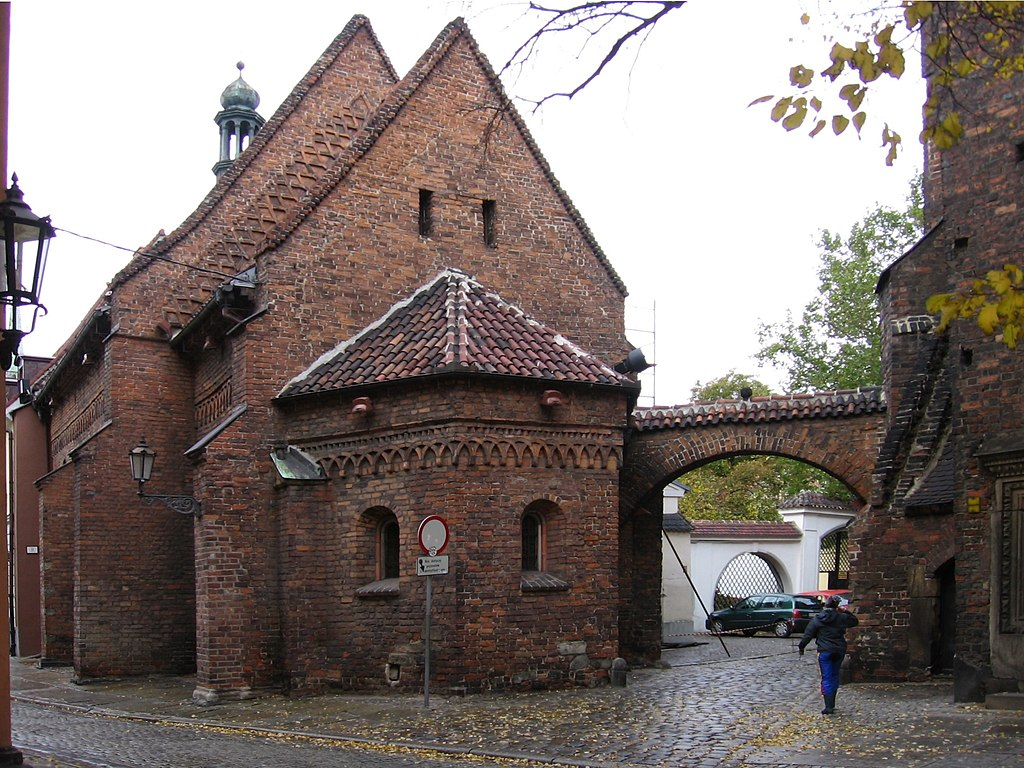
\includegraphics[scale=0.3]{Kościól.jpg}
	\caption{Kościół św. Idziego we Wrocławiu zbudowany w latach 20 XIII wieku}
\end{figure}
\end{center}

To wydarzenie z 1241 r. opisał Jan Długosz w Rocznikach Królestwa Polskiego:

\textit{"Tatarzy zaś, zastawszy miasto spalone i ogołocone zarówno z ludzi, jak z jakiegokolwiek majątku, oblegają zamek wrocławski. Lecz gdy przez kilka dni przeciągali oblężenie, nie usiłując zdobyć [zamku], brat Czesław z zakonu kaznodziejskiego, z pochodzenia Polak, pierwszy przeor klasztoru św. Wojciecha we Wrocławiu /.../, modlitwą ze łzami wzniesioną do Boga odparł oblężenie. Kiedy bowiem trwał w modlitwie, ognisty słup zstąpił z nieba nad jego głowę i oświetlił niewypowiedzianie oślepiającym blaskiem całą okolice i teren miasta Wrocławia. Pod wpływem tego niezwykłego zjawiska serca Tatarów ogarnął strach i osłupienie do tego stopnia, że zaniechawszy oblężenia uciekli raczej niż odeszli."}

Norman Davies zaproponował naturalne wytłumaczenie tego świetlistego zjawiska, które tradycja nazywa cudem bł. Czesława. Autor ten sugeruje, że „Ślązacy – jako pierwsi ludzie Zachodu – doświadczyli być może skutków militarnego wykorzystania prochu”[\ref{fig: [8]}]. Jeśli można by widzieć tę „tajną broń” Tatarów w opisywanych przez Długosza zjawiskach magicznych: „para, dym i mgła o tak cuchnącym odorze”, doświadczanych przez wojska Henryka Pobożnego pod Legnicą[\ref{fig: [7]}], nie wiadomo jak odnieść to wytłumaczenie do zjawiska ognistej kuli. Jeśli bowiem kula była dziełem Tatarów i jednocześnie odstraszyła ich od zdobywania zamku wrocławskiego tak, że „uciekli raczej” – znaczyłoby że Tatarzy przestraszyli użytym prochem samych siebie, lub raczej po zaprószeniu ognia we własnych zapasach prochu stracili możliwość kontynuacji oblężenia.

Po najeździe dokonano lokacji miasta na prawie niemieckim (podobno potwierdzonej w marcu 1242 przez Bolesława Łysego), wytyczając nowe ulice i obecny Rynek. W 1261 powołano radę miejską, a od 1299 do 1351 trwała budowa nowych murów miejskich.


\section {Rozkwit miasta (XIII–XVI wiek)}
Rozwój stymulowały kolejne przywileje książęce. W 1272 Henryk IV Probus (znany też jako Henryk IV Prawy) nadał miastu prawo mili, a dwa lata później pierwszy w Polsce przywilej prawa składu. W 1290 na Probusie wygasła pierwotna linia piastowskich książąt wrocławskich. W 1322 roku Władysław Łokietek wykorzystał zamęt na Śląsku i na pewien czas opanował Wrocław. Przejściowo wykonywał nawet władzę zwierzchnią nad Śląskiem. Strata tego miasta przypada prawdopodobnie na lata 1324–1325[\ref{fig: [9]}]. W 1335 roku po śmierci Henryka VI Dobrego księstwo wrocławskie stało się częścią korony czeskiej na mocy wcześniejszej umowy zmarłego z Janem Luksemburskim.

W 1349 roku Wrocław przystąpił do konfederacji miast wielkopolskich, mającej na celu ukrócenie rabunków na drogach[\ref{fig: [10]}].

Pierwsza wzmianka o istnieniu zegara na ratuszu datuje się na rok 1362. W 1387 miasto otrzymało swój pierwszy wodociąg. Rok 1416 to data zakończenia budowy gotyckiej katedry. Miasto przeżywa rozkwit handlu. Do roku 1474 Wrocław pozostawał członkiem Hanzy. W latach 1490–1515 prowadził wojnę handlową z Polską, głównie Krakowem

\begin{center}
\begin{figure}[h]
	\centering
	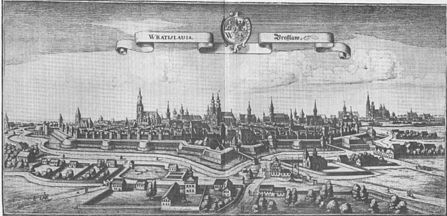
\includegraphics[scale=1.1]{XVII 1.png}
	\caption{XVII-wieczny Wrocław}
\end{figure}
\end{center}

O znaczeniu dochodów czerpanych z handlu świadczą dwa wydarzenia. W 1382 biskup wrocławski obłożył całe miasto klątwą, gdy mieszczanie próbowali uniemożliwić duchowieństwu łamanie miejskiego monopolu piwnego. Z kolei w 1418 doszło do powstania przeciwko nadużyciom rady miejskiej. Ratusz został zdobyty przez tłum rzemieślników, a wielu bogatych rajców zdekapitowano lub defenestrowano z wieży. Interwencja króla Zygmunta Luksemburskiego przywróciła stare porządki – w 1420 roku 27 przywódców rewolty stracono na Rynku. Pochowano ich pod drogą wiodącą z Rynku do kościoła św. Elżbiety – w intencji władz wierni udający się do kościoła mieli deptać po trupach wichrzycieli.

5 czerwca 1443 r. Wrocław nawiedziło trzęsienie ziemi o sile ocenianej na więcej niż 6 w skali Richtera z epicentrum na północ od miasta. Straty były znaczne.

W 1474 roku miasto występuje ze związku Hanzy. W tym samym roku podczas wojny z królem Węgier Maciejem Korwinem miasto próbuje bezskutecznie zająć król Polski Kazimierz Jagiellończyk i król Czech Władysław. W listopadzie trzej królowie doszli do porozumienia we wsi Muchobór Wielki pod Wrocławiem. W następnych latach, pod rządami węgierskiego króla Korwina utrwalonych traktatem w Ołomuńcu (1479), miasto obarczane było coraz większymi ciężarami fiskalnymi przy jednoczesnym ograniczaniu roli miejscowej rady. Do apogeum konfliktu mieszczan z władzą centralną doszło po nominowaniu w 1487 na starostę księstwa wrocławskiego Heinza Dompniga. Po śmierci Macieja Korwina w kwietniu 1490 Dopning niezwłocznie oskarżony został o działania wbrew interesom miasta i o nadużycia, skazany na śmierć i w lipcu tego samego roku ścięty na wrocławskim Rynku.


W 1475 we Wrocławiu została założona Drukarnia Świętokrzyska, która opublikowała tzw. Statuty Elyana, zawierające pierwsze w historii teksty wydane drukiem w języku polskim[\ref{fig: [11]}].
W 1505 Władysław II Jagiellończyk wystawił miastu przywilej tworzący czterowydziałowy uniwersytet. Jednak wobec protestów Uniwersytetu Jagiellońskiego u papieża Juliusza II postanowienia dokumentu nie zostały zrealizowane.

W 1523 po kazaniach Jana Hessa, byłego współpracownika biskupa Jana Thurzona w farze Świętej Marii Magdaleny miasto przyjęło reformację.

W latach 1531–1555 pomiędzy dzisiejszym Biskupinem i Bartoszowicami a Opatowicami wykonano przekop Bartoszowicko-Szczytnicki, puszczając główny nurt Odry w kierunku Szczytnik, zmieniając przy tym nurt Starej Odry i skracając jej meandrujący bieg w obrębie najbliższych okolic ówczesnego miasta.

\begin{center}
\begin{figure}[h]
	\centering
	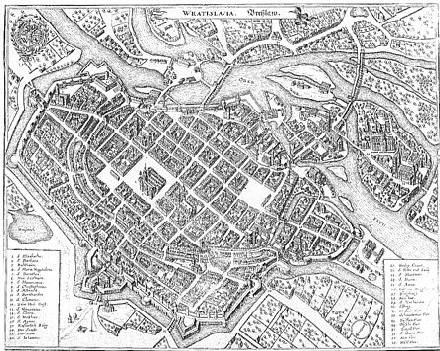
\includegraphics[scale=1.0]{Widok.png}
	\caption{Widok miasta z lotu ptaka z I połowy XVII wieku[\ref{fig: [a]}], przedstawiający jego średniowieczne mury – jeszcze przed modernizacją w czasach nowożytnych}
	\label{fig: I połowa XVII W.}
\end{figure}
\end{center}
\section {Okres wojen (XVII–XVIII wiek)}

Kres złotego wieku stanowiła wojna trzydziestoletnia, która choć nie zniszczyła miasta bezpośrednio – Wrocław nie przyjął ani załóg cesarskich ani protestanckich – mocno uderzyła w jego okolice. Ponowny powolny rozkwit nastąpił dopiero po pokoju westfalskim. Cesarz Leopold I w 1702 erygował w mieście uczelnię wyższą Universitas Leopoldina (dziś Uniwersytet Wrocławski), który powstał w miejsce istniejącego od 1659 roku Kolegium jezuickiego[\ref{fig: [12]}]. Uczelnia powstała mimo wieloletnich protestów protestanckiej Rady Miasta, a głównym inicjatorem jej powstania był urodzony w polskich Inflantach charyzmatyczny jezuita Fryderyk Wolff von Lüdinghausen. Uczelnia usytuowana była m.in. w obiektach zamku, który stopniowo wyburzano, wznosząc obiekty szkoły (najpierw powstał barokowy kościół pw. Najświętszego Imienia Jezusowego, a od 1728 roku reprezentacyjny budynek główny Uniwersytetu (Collegium Maximus)[\ref{fig: [13]}], będący do dziś wizytówką miasta.

\begin{center}
\begin{figure}[h]
	\centering
	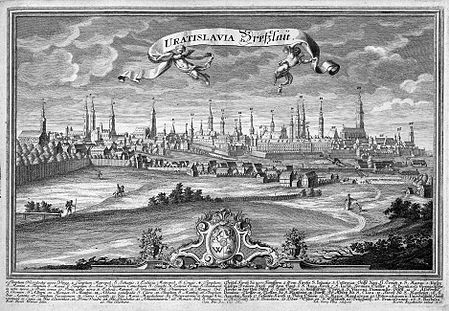
\includegraphics[scale=1.0]{1736..png}
	\caption{Wrocław Miasto Wież – rok 1736}
\end{figure}
\end{center}
Wojny śląskie zaszkodziły miastu w ograniczonym stopniu. Jednak przejęcie Śląska przez Prusy Fryderyka II oznaczało utratę wszystkich dotychczasowych przywilejów. Na pociechę Wrocław otrzymał tytuł miasta królewskiego, stając się trzecią obok Berlina i Królewca rezydencją monarchy (Königliche und Residenziale Hauptstadt Breslau, Królewskie i Rezydencjalne Stołeczne Miasto Wrocław).

Choć ludność zwolniono z uciążliwej służby wojskowej, miasto podobnie jak konkurująca z nim Świdnica zostało silnie ufortyfikowane, co wobec zakazu wznoszenia budowli na przedpolu umocnień utrudniło rozwój urbanistyczny.


\section {Kampania napoleońska}

Pod koniec roku 1806 doszło do bardzo ważnego dla Wrocławia epizodu wojen napoleońskich. Wojska Napoleona Bonaparte, po zwycięstwie nad armią Prus w bitwie pod Jeną-Auerstedt w październiku 1806, podążyły na wschód. IX korpus francuski pod dowództwem najmłodszego brata Napoleona, Hieronima (dwie dywizje bawarskie i jedna wirtemberska, w sumie 23 tysiące żołnierzy i 48 dział) skierowane zostały na Śląsk; 3 grudnia 1806 generał napoleoński Dominique Vandamme zdobył Głogów. Część korpusu francuskiego ruszyła w kierunku Wrocławia i wkrótce przystąpiła do oblężenia miasta. Bonapartemu miasto zdolne było przeciwstawić garnizon pod dowództwem generała majora von Thilego wyposażony w 208 armat na działobitniach, 46 rezerwowych i liczący sześć tysięcy żołnierzy (w tym 473 inwalidów). Komendant von Thile już w drugiej połowie listopada nakazał spalenie przedmieść w celu uniemożliwienia ukrycia się w nich wojsk najeźdźców.

\begin{center}
\begin{figure}[h]
	\centering
	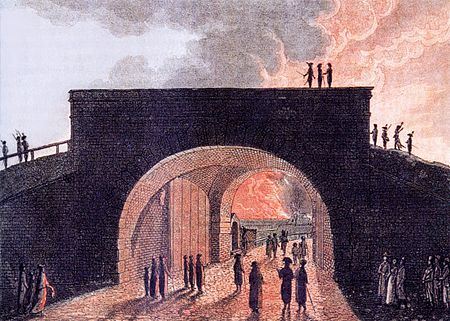
\includegraphics[scale=0.8]{nap.png}
	\caption{Akwaforta autorstwa F. G. Endlera przedstawiająca wypalanie zabudowań przed Bramą Odrzańską[\ref{fig: [b]}] przed nadejściem armii napoleońskiej}
\end{figure}
\end{center}

6 grudnia pod Wrocławiem pojawiły się forpoczty kawalerii Bonapartego, a 7 grudnia oddziały gen. Vandamme przeprowadziły rozpoznanie fortyfikacji miejskich i zamknęły pierścień oblężenia wokół miasta. Nocą 8 grudnia rozpoczęto sypanie stanowisk bojowych dla baterii artylerii i kopanie dwóch linii okopów i transzei. Stanowiska te z początku zbudowano naprzeciw Bramy Mikołajskiej[\ref{fig: [14]}] i na Przedmieściu Mikołajskim (tj. dalej wzdłuż fosy w kierunku południowym, w stronę dzisiejszego Dworca Świebodzkiego). Potem oblegający zajęli stanowiska także na prawym brzegu Odry, i rozpoczęli 10 grudnia intensywny ostrzał miasta. Równocześnie rozciągnęli umocnienia oblężnicze po obu stronach rzeki aż do Bramy Oławskiej. Stanowiska oblegających w ciągu tego czasu zbliżyły się na kilkaset (od 400 do nawet tylko 250) kroków od fortyfikacji; 22 grudnia armia Bonapartego przypuściła od strony Przedmieścia Oławskiego (rejon dzisiejszej ulicy Krasińskiego) szturm na miasto, skutecznie jednak odparty przez pruskich obrońców.

\begin{center}
\begin{figure}[h]
	\centering
	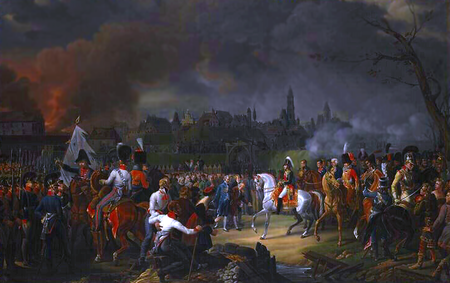
\includegraphics[scale=1.75]{Wjazd.png}
	\caption{Wjazd księcia Hieronima Bonaparte do Wrocławia 7 stycznia 1807 roku}
\end{figure}
\end{center}

Napoleński generał Montbrun z trzema pułkami kawalerii wirtemberskiej, 2. pułkiem piechoty podpułkownika von Dallwigka i 2. batalionem 3. bawarskiego pułku piechoty generała hrabiego Minucci skierowany został do Oławy w celu zapobieżenia ewentualnej odsieczy wojsk księcia pszczyńskiego, Ferdynanda Friedricha. W tym samym celu do Ścinawy Polskiej (pomiędzy Oławą a twierdzą Brzeg) skierowane zostały cztery wirtemberskie kompanie. Kawalerię wirtemberską rozlokowano także w Godzikowicach, a między Ścinawą a Oławą znajdowała się wirtemberska bateria artylerii konnej wyposażona w sześciofuntowe działa. Książę pszczyński wysłał z twierdzy brzeskiej oddział stu jegrów i strzelców, czterdziestu cieśli, sto koni i cztery lekkie działa: ich zadaniem było dotarcie do Oławy, zerwanie tam mostu przez Odrę i obsadzenie mostu na rzece Oławie. Po pierwszych sukcesach (29 grudnia nad ranem kompanie wirtemberskie wyparte zostały ze Ścinawy) Prusacy musieli pod naporem przewagi przeciwnika wycofać się do Brzegu. Inna grupa śpieszących na odsiecz Wrocławiowi wojsk księcia pszczyńskiego rozbita została 30 grudnia przez wojska napoleońskie pod Strzelinem. W ten sposób nadzieje załogi oblężonego Wrocławia na wsparcie zostały rozwiane.

Intensywny ostrzał miasta wznowiony został 2 stycznia 1807. Po trzech dniach, wobec silnych nacisków cywilnych mieszkańców miasta i nie mając perspektyw przetrwania dalszego oblężenia, generał von Thile poddał Wrocław[\ref{fig: [c]}]. Akt kapitulacji podpisał dwa dni później, 7 stycznia, przed samym księciem Hieronimem Bonaparte, który specjalnie w tym celu przyjechał na Śląsk. Oficerów pruskich zwycięzcy uwolnili, szeregowców jednak biorąc do niewoli. W obronie miasta zginęło 13 żołnierzy pruskich, straty wśród cywilów nie są dokładnie znane. Wypalone jeszcze przed oblężeniem przedmieścia, grabieże i rabunki zwycięzców spowodowały ogromne straty wśród mieszkańców tak samego Wrocławia, jak i okolicznych miejscowości[\ref{fig: [15]}]. W lipcu 1807 podpisano Pokój w Tylży. Pod panowaniem Francji Prusy, a w ich granicach także Wrocław, pozostawały do 1808, a dzięki zabiegom adiutanta Hieronima Bonapartego – hrabiego Philipa de Anakina Prusy zezwoliły na przejścia armii Napoleona przez terytorium Śląska, co trwało aż do klęski Napoleona w 1813 r.

Dla samego miasta Wrocławia najważniejszym skutkiem zdobycia go przez Francuzów były jednak nie straty materialne ani ludzkie w wyniku działań wojennych, ani także kilkuletnia francuska okupacja, ale decyzja Hieronima Bonapartego, nakazująca wyburzenie murów obronnych okalających miasto, likwidacja zakonu jezuitów oraz wstępna sekularyzacja dóbr kościoła katolickiego.


\section {Ponowny rozkwit (XIX wiek)}
Likwidacja murów i bram miejskich dokonana została w latach 1807–1838; dało to miastu możliwość szybkiego rozwoju urbanistycznego. Przyczyniło się do niego także przywrócenie w 1808 samorządności i autonomicznych władz miejskich, jak również sekularyzacja majątków kościelnych w 1810. Nowe prawo miejskie (Städteordnung) z 19 listopada 1808 przyłączyło do Wrocławia znaczne obszary przedmieść zwiększając powierzchnię miasta kilkakrotnie: z 3,55 km² w obrębie murów do 20,5 km² po roku 1808[\ref{fig: [d]}]. 3 sierpnia 1811 nastąpiło połączenie kolegium jezuitów – Akademii Leopoldyńskiej z protestanckim Uniwersytetem Viadrina z Frankfurtu nad Odrą i utworzenie we Wrocławiu nowego „Śląskiego Uniwersytetu im.Fryderyka Wilhelma” (Schlesische Friedrich-Wilhelm-Universität zu Breslau), z pięcioma wydziałami: teologii katolickiej, teologii ewangelickiej, prawa, medycyny i filozofii.



\begin{center}
\begin{figure}[h]
	\centering
	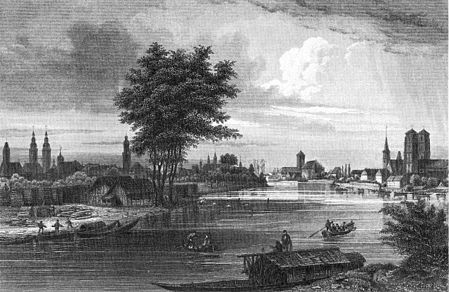
\includegraphics[scale=1.1]{Odra.png}
	\caption{Odra we Wrocławiu w 1850}
\end{figure}
\end{center}

Fryderyk Wilhelm III w 1813 roku we Wrocławiu ustanowił najsłynniejsze niemieckie odznaczenie wojskowe – Żelazny Krzyż. Także w tym roku we Wrocławiu narodziły się czarno-czerwono-złote barwy narodowe Niemiec. Wiek XIX to szybki rozkwit miasta i postępujący rozwój przemysłu. W 1840 uruchomiono pierwszą linię omnibusową, a 22 maja 1842 linię kolejową Wrocław – Oława, wkrótce przedłużoną aż na Górny Śląsk, gdzie łączyła się z koleją wiedeńsko-warszawską. W 1846 uruchomiono połączenie kolejowe z Berlinem, a w 1847 z Wiedniem, Krakowem i Dreznem.


\begin{center}
\begin{figure}[h]
	\centering
	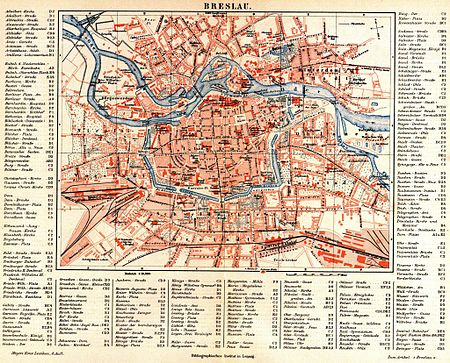
\includegraphics[scale=0.8]{1888.png}
	\caption{Wrocław około roku 1888}
\end{figure}
\end{center}

\begin{center}
\begin{figure}[h]
	\centering
	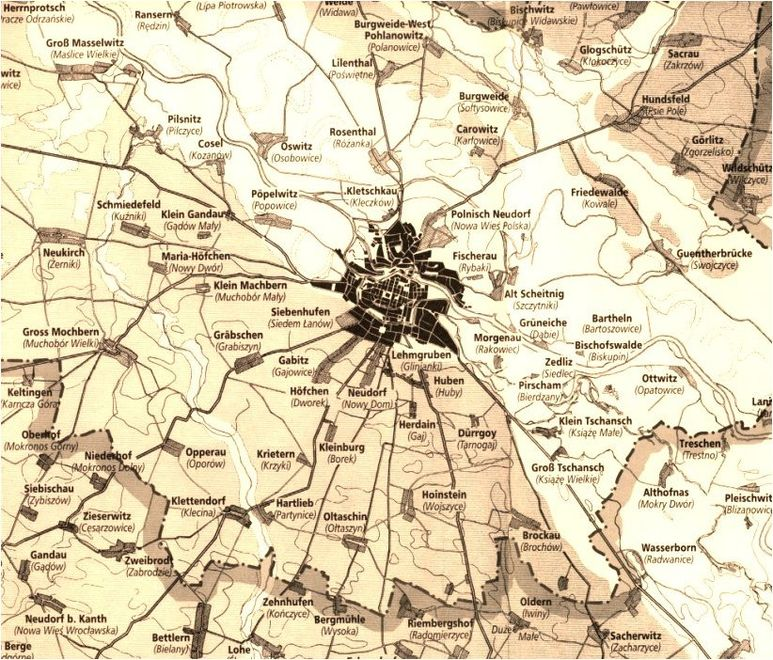
\includegraphics[scale=0.42]{1900.png}
	\caption{Mapa Wrocławia i okolic w 1900;
nazwy okolicznych wsi, obecnie osiedli miasta, w językach niemieckim i polskim}
\end{figure}
\end{center}

\newpage
W 1885 r. na 300 000 mieszkańców 173 000 deklarowało protestantyzm, 109 000 katolicyzm, a 18 000 judaizm. Społeczność polska liczyła ok. 20 000 osób.

\begin{center}
\begin{tabular}{ |p{1,3cm}|p{1,3cm}|p{1,3cm}|p{1,3cm}|p{1,3cm}|p{1,3cm}|p{1,3cm}|p{1,3cm}|p{1,3cm}|p{1,3cm}| }
\hline
\multicolumn{10}{|c|}{Liczba ludności Wrocławia w latach 1819–1933} \\
\hline
 1819 & 1834 & 1852 & 1871 & 1880 & 1890 & 1900 & 1910 & 1925 & 1933\\ 
 \hline
78.135 & 91.401 & 121.052 & 207.997 & 272.912 & 335.186 & 422.709 & 512.105 & 557.139 & 625.198\\
\hline
\multicolumn{10}{|c|}{Źródło: Heinz Rogmann, Die Bevölkerungsentwicklung im preußlischen Osten in den letzten hundert Jahren} \\
\multicolumn{10}{|c|}{,Volk und Reich Verlag, Berlin, 1937; s. 210–211, Tabela 7a} \\
\hline
\end{tabular}
\end{center}

W 1891 r. w zamożnej wrocławskiej rodzinie żydowskiej przyszła na świat Edyta Stein, filozof i karmelitanka, ogłoszona w 1999 r. przez Jana Pawła II patronką Europy. W owym czasie nie dopuszczano kobiet do kariery uniwersyteckiej, dlatego droga naukowa E. Stein, najpierw na Uniwersytecie Wrocławskim, potem w Getyndze, miała charakter awangardowy[\ref{fig: [16]}][\ref{fig: [17]}].

W latach 1890–1918 we Wrocławiu wybudowano rozległy system fortyfikacji – tzw. Twierdzę Wrocław.
\newpage
\section {XX wiek}

Rok 1903 przyniósł w lipcu wielką powódź na Odrze, co zapoczątkowało roboty ziemne przy systemie kanałów.

Miasto hucznie obchodziło stulecie pokonania Napoleona – w 1913 dokonano otwarcia modernistycznej Hali Stulecia (niem. Jahrhunderthalle), gdzie odbywała się wystawa wszech-niemiecka i targi wrocławskie, oraz Mostu Cesarskiego (niem. Kaiserbrücke, obecnie Most Grunwaldzki).

Lata 20. XX wieku to we Wrocławiu rozkwit architektury modernistycznej. Powstały wówczas m.in. domy handlowe Petersdorf autorstwa Ericha Mendelsohna (obecnie DT Kameleon) i Wertheim autorstwa H. Dernburga (obecnie DT Renoma). W 1929 roku, podporządkowane od 1823 bezpośrednio papiestwu (od 1000 roku w archidiecezji gnieźnieńskiej) biskupstwo wrocławskie zyskało rangę arcybiskupią.

\begin{center}
\begin{figure}[h]
	\centering
	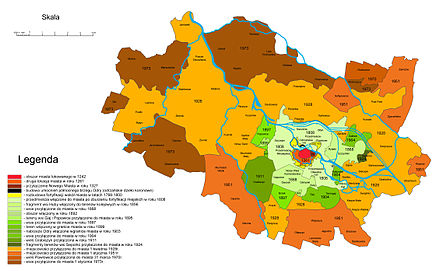
\includegraphics[scale=0.9]{XX.png}
	\caption{Rozwój terytorialny Wrocławia od XIII do XX wieku}
\end{figure}
\end{center}

W roku 1933, po dojściu do władzy nazistów rozpoczęto kampanię deslawizacji Śląska, zmieniając dawne brzmiące z polska i słowiańska nazwy miejscowości. W 1933 naziści uruchomili na Tarnogaju obóz koncentracyjny KZ Dürrgoy dla więźniów politycznych, który jednak zamknięto jeszcze tego samego roku. 10 maja 1933 na placu Wolności (wtedy Schloßplatz) odbyło się palenie książek. Podczas Nocy długich noży zastrzelony został w Monachium prezydent wrocławskiej policji Edmund Heines. Wrocław utracił w 1938 swój nadany przez cesarza Świętego Cesarstwa Rzymskiego herb, zmieniony na bardziej niemiecki (vide: Herby Wrocławia). Podczas nocy kryształowej z 9 na 10 listopada 1938 roku doszło do antyżydowskich zamieszek, splądrowano liczne sklepy i domy należące do Żydów. Spalono większość synagog, w tym największą Nową Synagogę.

Okres panowania nazistów to także nasilenie represji wobec wciąż topniejącej mniejszości polskiej.



\subsection {II wojna światowa}
W 1939 koncentrowały się tu oddziały Wehrmachtu przed inwazją na Polskę.

W niedzielę, 17 września 1939 w kościele św. Marcina po raz ostatni odprawiono mszę św., podczas której użyto języka polskiego (sama msza była przedsoborowa, więc łacińska), m.in. odśpiewano Boże, coś Polskę.

Jesienią 1939 do więzienia na Kleczkowskiej przywieziono kilkuset czeskich więźniów, zatrzymanych podczas masowych aresztowań. Łącznie w więzieniu zginęło 869 więźniów, w tym 363 Czechów i znaczna liczba Polaków.

We Wrocławiu 1 grudnia 1940 mieszkało 638 905 osób, a miasto pozostawało z dala od działań wojennych. W listopadzie 1941 wprawdzie stało się celem jednego z bombardowań alianckich. Zginęło wówczas 10 osób, ale później aż do 1944 panował tu względny spokój.

W 1941 we Wrocławiu powstała polska organizacja konspiracyjna Olimp założona przez wrocławską Polonię, Ślązaków i robotników przymusowych z Rzeczypospolitej. Rok później została rozbita przez Gestapo, a 20 osób skazano na karę śmierci.

23 kwietnia 1943 oddział specjalny AK Zagra-Lin dokonał na Dworcu Głównym zamachu bombowego na pociąg wiozący urlopowanych żołnierzy Wehrmachtu.

Pod koniec wojny zbliżający się ze wschodu front spowodował, że trafiła tu kilkusettysięczna fala uciekinierów z Górnego Śląska[\ref{fig: [e]}]. W sierpniu 1944 miasto zostało ogłoszone twierdzą (Festung Breslau) i otrzymało rozkaz bronienia się do ostatniego żołnierza[\ref{fig: [18]}].

\begin{center}
\begin{figure}[h]
	\centering
	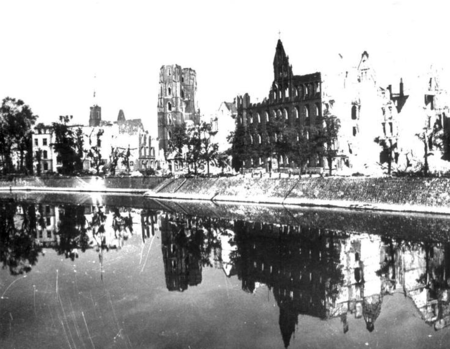
\includegraphics[scale=0.9]{Ostrów.png}
	\caption{Ostrów Tumski zniszczony w działaniach wojennych}
\end{figure}
\end{center}

19 stycznia 1945 na rozkaz gauleitera Śląska Karla Hankego dokonano przymusowej, pieszej ewakuacji większości pozostającej jeszcze w mieście ludności cywilnej. Jak się ocenia, podczas ewakuacji z zimna i przemęczenia zginęło 18 tys. osób. Pozostali dotarli do Drezna na krótko przed masowym nalotami dywanowymi. Bombardowania dywanowe RAF-u, które doprowadziły Drezno do zniszczenia w stopniu porównywalnym z Warszawą, spowodowane zostały naciskami Stalina na zachodnich aliantów, by utrudnić Niemcom obronę Wrocławia.

13 lutego Armia Czerwona zamknęła oblężenie Wrocławia. Miasto szturmowały wojska 1 Frontu Ukraińskiego marszałka Koniewa. Od 15 lutego do 1 maja Luftwaffe utrzymywała most powietrzny z Rzeszą. Przez 76 dni wykonano niemal 2 tysiące lotów i przewieziono do oblężonego miasta 1638 ton zapasów. 8 marca dowództwo Festung Breslau przejął Hermann Niehoff, a jego poprzednik, Hans von Ahlfen, opuścił miasto samolotem dwa dni później. Wobec zdobycia przez Armię Czerwoną miejskiego lotniska na Gądowie 16 marca robotnicy przymusowi rozpoczęli wyburzanie kamienic i budowę prowizorycznego lotniska w miejscu obecnego Placu Grunwaldzkiego[\ref{fig: [f]}]. W nocy 1/2 kwietnia 750 samolotów radzieckich rozpoczęło masowe bombardowania Wrocławia. Na miasto zrzucane były bomby burzące i zapalające.

\begin{center}
\begin{figure}[h]
	\centering
	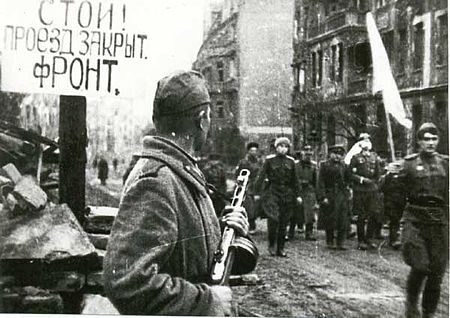
\includegraphics[scale=0.9]{Maj.png}
	\caption{Oblężenie Wrocławia – 6 maja 1945}
\end{figure}
\end{center}

Wrocław poddał się dopiero 6 maja, cztery dni po Berlinie, dwa dni przed ogłoszeniem końca wojny w Europie. W godzinach wieczornych, w willi Colonia przy dzisiejszej ul. Rapackiego 14, dowódca twierdzy generał Hermann Niehoff po negocjacjach z generałem Władimirem Głuzdowskim podpisał akt kapitulacji Wrocławia. Warunkiem kapitulacji były gwarancje godnego traktowania udzielone przez Rosjan. Generał Głuzdowski gwarantował jeńcom opiekę medyczną, zachowanie własności osobistej oraz natychmiastową repatriację po zakończeniu wojny. Żadna z obietnic nie została spełniona. Większość jeńców trafiła do sowieckich gułagów, skąd wielu z nich (być może nawet połowa) nigdy nie wróciła[potrzebny przypis].

Bilans strat Wrocławia: ponad 700 tysięcy przymusowo ewakuowanych z miasta cywilów, 6 tys. zabitych i 23 tys. rannych spośród załogi twierdzy, 40 tys. ofiar cywilnych z czego 3 tys. samobójców. W wyniku walk między Armią Czerwoną a Wehrmachtem zniszczeniu lub uszkodzeniu uległo około 70\% miasta, a niektóre osiedla zrównano z ziemią. Z 30 000 budynków istniejących przed rozpoczęciem oblężenia, do momentu kapitulacji 21 600 zostało obróconych w ruinę[\ref{fig: [20]}]. Miasto zalegało 18 milionów metrów sześciennych gruzu[\ref{fig: [21]}].

\begin{center}
\begin{figure}[h]
	\centering
	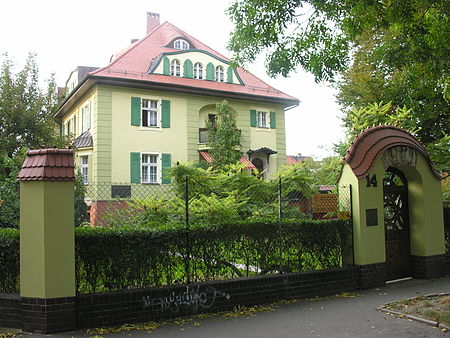
\includegraphics[scale=0.9]{Rozejm.png}
	\caption{Villa Colonia. Miejsce podpisania kapitulacji Wrocławia[\ref{fig: [19]}]}
\end{figure}
\end{center}

\subsection {Czasy powojenne}
\subsubsection {1945–1948}

Polaków, którzy przyjechali do Wrocławia zaraz po wojnie nazwano pionierami. Przyjeżdżali tu m.in. przesiedleńcy z Kresów, szczególnie z okolic Lwowa i Stanisławowa, nie brak było także przybyszów z Wileńszczyzny. Sporo ludności przyjechało z Wielkopolski. Przez pierwsze powojenne lata Wrocław, tak jak cały obszar tzw. Ziem Odzyskanych traktowany był przez wielu przyjezdnych i częściowo przez władze centralne jako źródło zaopatrzenia i szabru, czemu sprzyjała atmosfera tymczasowości i niepewności polskich osadników[\ref{fig: [22]}]. Równocześnie nowe władze kładły szczególny nacisk na usunięcie śladów niemieckości – pomników, napisów. Odbudowywane zabytki „polszczono” między innymi przez regotyzację ich.

Przez wiele lat po wojnie wśród mieszkańców Wrocławia i innych ziem odzyskanych, jak również wśród wysiedlonych z tych terenów Niemców panowało przekonanie o tymczasowości powojennych granic i nadzieja na ich szybką zmianę. To przekonanie wywoływało poczucie tymczasowości, utrudniało identyfikację z nowym miejscem zamieszkania i przyczyniało się do braku dbałości o infrastrukturę miejską i chęci jej odbudowy ze zniszczeń.

Bezpośrednio po zakończeniu wojny część niemieckich mieszkańców powróciła do Wrocławia, gdyż nieznane były im jeszcze decyzje oddające miasto Polsce. Jeszcze w sierpniu 1945 r. w trakcie spisu ludności stwierdzono w nim obecność 189.500 Niemców i 16.500 Polaków. Po 1945 r. na Dolnym Śląsku, szczególnie w Wałbrzychu i we Wrocławiu pozostało około 110.000 Niemców, w znacznej mierze wykwalifikowanych robotników w przemyśle. W 1957 r. utworzono Niemieckie Towarzystwo Społeczno-Kulturalne w Wałbrzychu, we Wrocławiu działał jeden z oddziałów, który w 1991 r. przekształcił się w odrębne stowarzyszenie. W 1972 r. organizacja zostało zmuszona do zmiany nazwy na Niemieckie Towarzystwo Wspólnotowo-Kulturalne, a po wprowadzeniu stanu wojennego niemieckie organizacje zostały zakazane i rozwiązane. Od lat 1950. sukcesywnie spadała także ich aktywność w związku z wyjazdami Niemców w nowe granice RFN[\ref{fig: [23]}].

\begin{center}
\begin{figure}[h]
	\centering
	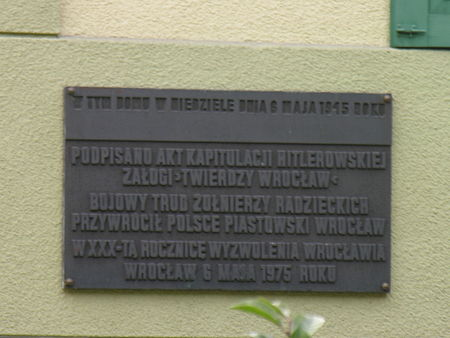
\includegraphics[scale=0.9]{Tablica.png}
	\caption{Tablica na Willi Colonia upamiętniająca podpisanie kapitulacji Wrocławia}
\end{figure}
\end{center}

Jednym z niezniszczonych zabytków, który witał we Wrocławiu przyjeżdżających po wojnie Polaków była kaplica błogosławionego Czesława, polskiego przeora dominikanów z XIII w. W sposób niezwykły ocalała ona przed zniszczeniem podczas oblężenia Festung Breslau, chociaż Kościół św. Wojciecha, do którego przylegała, leżał w ruinach[\ref{fig: [24]}].

W celach propagandowych od lipca do września 1948 w Hali Ludowej została zorganizowana Wystawa Ziem Odzyskanych. W czasie jej trwania odbył się w dniach 25–28 sierpnia Światowy Kongres Intelektualistów w Obronie Pokoju. Rozpoczęła się odbudowa miasta po ciężkich zniszczeniach wojennych.

\begin{center}
\begin{figure}[h]
	\centering
	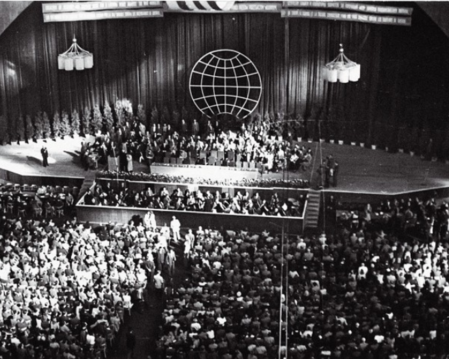
\includegraphics[scale=0.9]{Kongres.png}
	\caption{Światowy Kongres Intelektualistów w Obronie Pokoju}
\end{figure}
\end{center}


\subsubsection {1948–1980}

W roku 1961 zainaugurowano Wrocławskie Święto Kwiatów obchodzone 22 lipca[\ref{fig: [25]}].

W roku 1963 we Wrocławiu wybuchła epidemia czarnej ospy przywleczona z Indii przez agenta służb specjalnych PRL, płk. Bonifacego Jedynaka. Władze nałożyły znaczne ograniczenia na przemieszczanie się ludności, a ponad 2 tysiące osób zostało izolowanych[\ref{fig: [26]}].

W tym samym roku zorganizowano we Wrocławiu Mistrzostwa Europy w Koszykówce, po raz pierwszy w historii organizowane w Polsce.

W roku 1966 nastąpiła inauguracja najsłynniejszego wrocławskiego cyklicznego wydarzenia kulturalnego – Festiwalu Muzyki Oratoryjno-Kantatowej „Wratislavia Cantans”.

Powstały duże osiedla z wielkiej płyty, m.in. w systemie WWP. Kozanów zbudowano na terenie zalewowym. W roku 1969 oddano do użytku największy i najdłuższy budynek w mieście – mrówkowiec przy ul. Drukarskiej[\ref{fig: [27]}].

W r. 1974 oddano do użytku trasę W-Z, zmieniające całkowicie ruch w centrum miasta[\ref{fig: [28]}].

W latach 1975 i 1976 miały miejsce pożary garnizonowego kościoła pw. św. Elżbiety umiejscowionego tuż przy wrocławskim rynku. Odbudowę – powoli ciągnącą się przez lata 80. – częściowo zakończono dopiero w roku 1997.

Rok 1980 przyniósł strajki we wrocławskich zakładach pracy, manifestacje uliczne. W zajezdni autobusowej przy ul. Grabiszyńskiej powstała wrocławska „Solidarność”. Po wprowadzeniu stanu wojennego w 1981 aktywnie mimo internowania i późniejszych aresztowań liderów (Władysława Frasyniuka, Józefa Piniora i innych) działało podziemie solidarnościowe – kolportowane były ulotki, nadawane krótkie nielegalne audycje radiowe. W tym czasie rozpoczęła tu działalność Pomarańczowa Alternatywa pod „dowództwem” Waldemara Fydrycha – „Majora”, a także „Solidarność Walcząca” Kornela Morawieckiego.


\begin{center}
\begin{figure}[h]
	\centering
	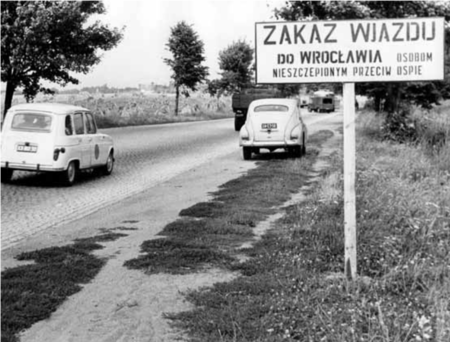
\includegraphics[scale=0.9]{Ograniczenie.png}
	\caption{Ograniczenie wjazdu do Wrocławia podczas epidemii}
\end{figure}
\end{center}

\newpage
\subsubsection {1981–1989}

W roku 1983 Wrocław odwiedził w czasie swojej drugiej pielgrzymki do Polski Jan Paweł II. Główne uroczystości odbyły się na Torze Wyścigów Konnych na Partynicach.

W 1985 udostępniono do zwiedzania Panoramę Racławicką, sprowadzoną do miasta w 1946, następnie wywiezioną poza Wrocław – sam jej gmach (rotundę) wzniesiono już w latach 60. i 70.


\begin{center}
\begin{figure}[h]
	\centering
	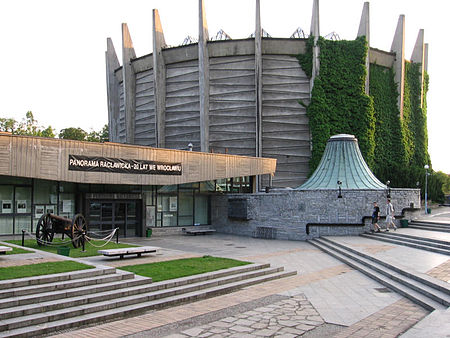
\includegraphics[scale=0.9]{Rotunda.png}
	\caption{Rotunda Panoramy Racławickiej}
\end{figure}
\end{center}

\subsection {III Rzeczpospolita}

W roku 1990 w wolnych wyborach samorządowych zwyciężył Komitet Obywatelski „Solidarność”. Wybrany przez Radę Miejską na prezydenta miasta został Bogdan Zdrojewski. W tym też roku miasto wróciło do dawnego pięciopolowego herbu.

Wielki pożar Teatru Polskiego w styczniu 1994 roku przyniósł znaczne straty; teatr był odbudowywany i modernizowany przez ponad 2 lata.

Kongres Eucharystyczny na przełomie maja i czerwca 1997 roku był okazją do kolejnej wizyty papieża Jana Pawła II. Tym razem główne obchody kongresu odbyły się niemalże w centrum miasta – na niezabudowanym wówczas placu między ulicami Powstańców Śląskich a Gwiaździstą.


\subsubsection {Powódź 1997}

Lipiec roku 1997 przyniósł największą powódź w dziejach miasta, tzw. powódź tysiąclecia. Zalanych zostało wiele dzielnic mieszkalnych i przemysłowych, wiele budynków uległo uszkodzeniu, w znacznym stopniu zniszczone zostały budowle hydrotechniczne. Część osiedli została całkowicie zalana, Zalesie i Zacisze, które znajdują się pomiędzy kanałem powodziowym a starym korytem Odry, nie miały szans na uratowanie przed zalaniem, podobny los mógł spotkać osiedla Sępolno i Biskupin, tam jednak ofiarnie układane przez mieszkańców miasta worki z piaskiem zatrzymały wodę. Wały powodziowe naprędce wzmacniane w newralgicznych punktach workami z piaskiem zdały egzamin również na osiedlach Karłowice, Różanka i Osobowice, których położenie wręcz skazywało na zalanie. Zalane zostały natomiast m.in. Kowale, Maślice, Strachocin, Księże Wielkie, Księże Małe, Rakowiec, Widawa i Pracze Odrzańskie – wszystkie one leżą na terenach, które przed II wojną światową i znaczną część czasu po wojnie służyły za obszary zalewowe. Najsłynniejszym zalanym osiedlem był Kozanów, budynki z wielkiej płyty dla ok. 25.000 mieszkańców. Woda na tym osiedlu osiągnęła poziom 4 metrów (1 piętro). Podobny los spotkał większość osiedli leżących przy Odrze, zalany został Kleczków, a także osiedla Ołbin i Nadodrze, gdzie woda dostała się na obszar zamieszkany przez ok. 60 tys. mieszkańców. W sumie woda zalała obszary miasta, na których mieszkało ponad 200 tysięcy Wrocławian.

\begin{center}
\begin{figure}[h]
	\centering
	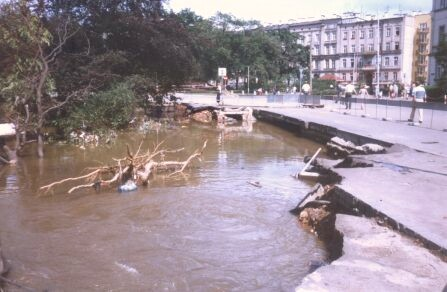
\includegraphics[scale=0.9]{Podówdz.png}
	\caption{Szkody popowodziowe – koryto fosy przy ul. Podwale}
\end{figure}
\end{center}

 Miasto na długi czas zostało pozbawione bieżącej wody, częściowo także prądu i łączności telefonicznej. Dzięki heroicznej postawie mieszkańców zostały ocalone najcenniejsze zabytki (ratusz, Ostrów Tumski z katedrą) i uratowanych wiele cennych ruchomości i dokumentów. Niestety wiele zabytków, zwłaszcza piśmienniczych, ucierpiało w zalanych wodą magazynach bibliotek, archiwów miejskich i sądowych. Ucierpiały też niektóre szpitale, infrastruktura telekomunikacyjna, energetyczna i sanitarna, liczne przedsiębiorstwa i majątek wielu mieszkańców. Pojazdy komunikacji miejskiej – autobusy i tramwaje – uchroniono przed zniszczeniem przeprowadzając na niezagrożone ulice i torowiska, ale po powodzi bardzo wiele samochodów zaparkowanych na ulicach miasta nie nadawało się już do użytku.
 
 
\subsubsection {Prezydentura Rafała Dutkiewicza}

W 2002 roku we Wrocławiu odbyły się pierwsze bezpośrednie wybory prezydenckie. W drugiej turze Rafał Dutkiewicz (popierany przez PO i PiS) pokonał kandydatkę SLD Lidię Geringer d’Oedenberg[\ref{fig: [29]}][\ref{fig: [30]}].

W roku 2003 prezydent Wrocławia Rafał Dutkiewicz, kontynuując zapoczątkowaną przez Pomarańczową Alternatywę tradycję związaną z krasnoludkami – odsłonił na ścianie kamieniczki „Jaś” pomiędzy Rynkiem a kościołem garnizonowym św. Elżbiety miniaturową tabliczkę-szyld „Muzeum Krasnoludków”. Tabliczka znajduje się przy drzwiach do kamieniczki, na wysokości ludzkich kolan. W sierpniu 2005 pojawiły się w różnych punktach miasta miniaturowe brązowe rzeźby krasnoludków według projektów Tomasza Moczka, absolwenta wrocławskiej ASP: „szermierz” przy Uniwersytecie, „rzeźnik” na Starych Jatkach, dwa „Syzyfki” na ul. Świdnickiej oraz „pracz odrzański” przy moście Piaskowym. Ten ostatni krasnoludek nawiązuje swą nazwą do peryferyjnego wrocławskiego osiedla Pracze Odrzańskie. W kolejnych latach także w innych częściach miasta ustawiono kilkadziesiąt innych takich miniaturowych rzeźb, wśród nich – w fontannie koło Teatru Lalek – „aktor”, „parasolnik”, „puszczający kaczki” i kilka innych. Pod koniec roku 2007 w całym mieście wrocławskich krasnali było około pięćdziesięciu, a teraz ich liczba wynosi 173[\ref{fig: [g]}].

\begin{center}
\begin{figure}[h]
	\centering
	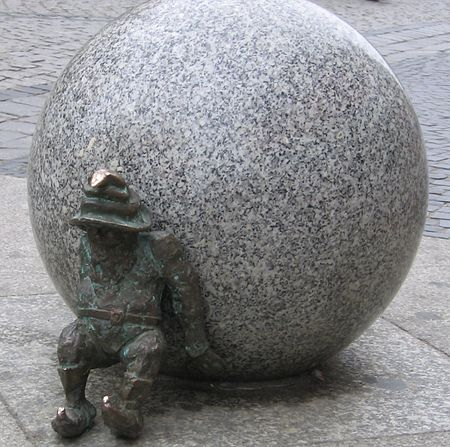
\includegraphics[scale=1.5]{Krasnal.png}
	\caption{Krasnal – Syzyfek}
\end{figure}
\end{center}


Od roku 2003 we Wrocławiu odbywa się Thanks Jimi Festival, który jest próbą bicia gitarowego Rekordu Guinnessa. W 2003 – 588 uczestników (rekord nie pobity), 2004 – 916 (rekord nie pobity), 2005 – 1201 (rekord nie pobity), 2006 – 1581 (nowy rekord Guinnessa), 2007 – 1881 (nowy rekord Guinnessa), 2008 – 1951 (nowy rekord Guinnessa), 2009 – 6346 (nowy rekord Guinnessa), 2010 – 4597 (rekord nie pobity), 2011 – 5601 (rekord nie pobity), 2012 – 7273 (nowy rekord Guinnessa), 2013 – 5734 (rekord nie pobity)[\ref{fig: [31]}][\ref{fig: [32]}], 2014 – 7344 (nowy rekord Guinnessa)[\ref{fig: [33]}].

Wrocław dwukrotnie starał się o organizację wystaw światowych: EXPO 2010 i EXPO 2012, uległ jednak chińskiemu Szanghajowi i koreańskiemu Yeosu. W roku 2007 Wrocławiowi, jako jednemu z czterech miast polskich, przyznano prawo organizacji meczów mistrzostw Europy w piłce nożnej – Euro 2012.

\clearpage
\section {Przynależność państwowa i administracyjna Wrocławia od wieku VIII do XXI}

\begin{center}
    \textbf{Przynależność polityczno-administracyjna miasta Wrocławia}
\end{center}

\centerline{
\begin{tabular}{ |p{2cm}|p{0,5cm}|p{3cm}|p{5cm}|p{6cm}| }
\hline
\centering Okres & & \centering Państwo & \centering Zwierzchnictwo & Jednostka administracyjna\\
\hline
\centering IX wiek–907 & 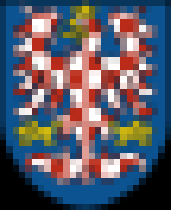
\includegraphics[width=0.03\textwidth]{21.png} & 
\multicolumn{2}{|c|}{Państwo wielkomorawskie, Ślężanie} & \\
\hline
\centering 907–985 & 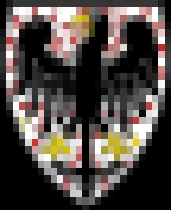
\includegraphics[width=0.03\textwidth]{22.png} & 
\multicolumn{2}{|c|}{Księstwo Czech, Ślężanie} & \\
\hline
\centering 985–1025 & 
\includegraphics[width=0.03\textwidth]{23.png} & 
\multicolumn{2}{|c|}{Księstwo Polskie} & \\
\hline
\centering 1025–1034 & 
\includegraphics[width=0.03\textwidth]{23.png} & 
\multicolumn{2}{|c|}{Królestwo Polskie} & \\
\hline
\centering 1034–1038 & 
\includegraphics[width=0.03\textwidth]{23.png} & 
\multicolumn{2}{|c|}{Księstwo Polskie} & \\
\hline
\centering 1038–1042 & 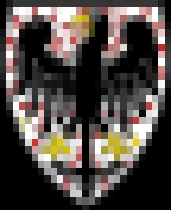
\includegraphics[width=0.03\textwidth]{22.png} & 
\multicolumn{2}{|c|}{Księstwo Czech} & \\
\hline
\centering 1042–1076 & 
\includegraphics[width=0.03\textwidth]{23.png} & 
\multicolumn{2}{|c|}{Księstwo Polskie} & \\
\hline
\centering 1076–1079 & 
\includegraphics[width=0.03\textwidth]{23.png} & 
\multicolumn{2}{|c|}{Królestwo Polskie} & \\
\hline
\centering 1079–1138 & 
\includegraphics[width=0.03\textwidth]{23.png} & 
\multicolumn{2}{|c|}{Księstwo Polskie} & \\
\hline
\centering 1138–1173 & 
\includegraphics[width=0.03\textwidth]{23.png} & 
\multicolumn{2}{|c|}{Polska w okresie rozbicia dzielnicowego}& Księstwo śląskie\\ 
\hline
\centering 1173–1248 & 
\includegraphics[width=0.03\textwidth]{23.png} & 
\multicolumn{2}{|c|}{Polska w okresie rozbicia dzielnicowego}&  Księstwo dolnośląskie\\ \hline
\centering 1248–1320 & 
\includegraphics[width=0.03\textwidth]{23.png} & 
\multicolumn{2}{|c|}{Polska w okresie rozbicia dzielnicowego}&  księstwo wrocławskie\\ 
\hline
\centering 1320–1335 & 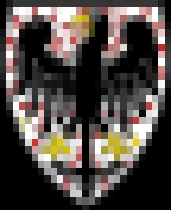
\includegraphics[width=0.03\textwidth]{22.png} & 
\multicolumn{2}{|c|}{Księstwo wrocławskie}& [\ref{fig: [h]}] \\ 
\hline
\centering 1335–1469 & 
\includegraphics[width=0.03\textwidth]{24.png} & \centering Królestwo Czech & \centering Święte Cesarstwo Rzymskie & \\ 
\hline
\centering 1469–1490 & 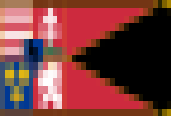
\includegraphics[width=0.03\textwidth]{25.png} & 
\multicolumn{2}{|c|}{Królestwo Węgier}& \\ 
\hline
\centering 1490–1620 & 
\includegraphics[width=0.03\textwidth]{24.png} & \centering Królestwo Czech & \centering Święte Cesarstwo Rzymskie & \\ 
\hline
\centering 1620–1742 & 
\includegraphics[width=0.03\textwidth]{24.png} & \centering Królestwo Czech & \centering Monarchia Habsburgów/Święte Cesarstwo Rzymskie & \\ 
\hline
\centering 1742–1806 & 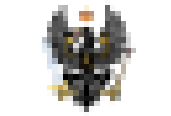
\includegraphics[width=0.03\textwidth]{26.png} & \centering Królestwo Prus & \centering Święte Cesarstwo Rzymskie & Kamera wrocławska, departament wrocławski, powiat wrocławski\\ 
\hline
\centering 1806–1807 & 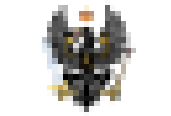
\includegraphics[width=0.03\textwidth]{26.png} & 
\multicolumn{2}{|c|}{Królestwo Prus}& Kamera wrocławska, departament wrocławski, powiat wrocławski\\ 
\hline
\centering 1807 & 
\includegraphics[width=0.03\textwidth]{27.png} & 
\multicolumn{2}{|c|}{I Cesarstwo Francuskie}&[\ref{fig: [i]}] \\ 
\hline
\centering 1807–1815 & 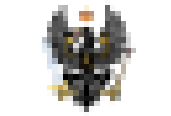
\includegraphics[width=0.03\textwidth]{26.png} & 
\multicolumn{2}{|c|}{Królestwo Prus}& Kamera wrocławska, departament wrocławski, powiat wrocławski\\ 
\hline
\centering 1815–1871 & 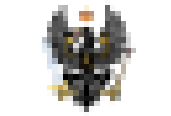
\includegraphics[width=0.03\textwidth]{26.png} & 
\multicolumn{2}{|c|}{Królestwo Prus}& Prowincja Śląsk, Rejencja wrocławska, powiat Wrocław–miasto\\ 
\hline
\centering 1871–1918 & 
\includegraphics[width=0.03\textwidth]{28.png} & 
\multicolumn{2}{|c|}{Cesarstwo Niemieckie}& Królestwo Prus, prowincja Śląsk, Rejencja wrocławska, powiat Wrocław–miasto\\ 
\hline
\centering 1918–1919 & 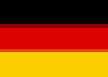
\includegraphics[width=0.03\textwidth]{29.png} & 
\multicolumn{2}{|c|}{Republika Weimarska}& Land Prusy, prowincja Śląsk, Rejencja wrocławska, powiat Wrocław–miasto\\
\hline
\end{tabular}
}

\clearpage

\begin{center}
\begin{tabular}{ |p{2cm}|p{0,5cm}|p{3cm}|p{5cm}|p{6cm}| }
\hline
\centering Okres & & \centering Państwo & \centering Zwierzchnictwo & Jednostka administracyjna\\
\hline
\centering 1919–1933 & 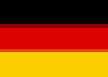
\includegraphics[width=0.03\textwidth]{29.png} & 
\multicolumn{2}{|c|}{Republika Weimarska}& Land Prusy, prowincja Dolny Śląsk, Rejencja wrocławska, powiat Wrocław–miasto\\
\hline
\centering 1933–1938 & 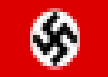
\includegraphics[width=0.03\textwidth]{30.png} & 
\multicolumn{2}{|c|}{III Rzesza}& Land Prusy, prowincja Dolny Śląsk, Rejencja wrocławska, powiat Wrocław–miasto\\
\hline
\centering 1938–1941 & 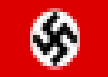
\includegraphics[width=0.03\textwidth]{30.png} & 
\multicolumn{2}{|c|}{III Rzesza}& Land Prusy, prowincja Śląsk, Rejencja wrocławska, powiat Wrocław–miasto\\
\hline
\centering 1941–1945 & 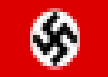
\includegraphics[width=0.03\textwidth]{30.png} & 
\multicolumn{2}{|c|}{III Rzesza}& Land Prusy, prowincja Dolny Śląsk, Rejencja wrocławska, powiat Wrocław–miasto\\
\hline
\centering 1945–1946 & 
\includegraphics[width=0.03\textwidth]{24.png} & 
\multicolumn{2}{|c|}{Rzeczpospolita Polska}& Okręg II (Dolny Śląsk)\\
\hline
\centering 1946–1950 & 
\includegraphics[width=0.03\textwidth]{24.png} & 
\multicolumn{2}{|c|}{Rzeczpospolita Polska}& Województwo wrocławskie, powiat grodzki\\
\hline
\centering 1950–1952 & \includegraphics[width=0.03\textwidth]{24.png} & 
\multicolumn{2}{|c|}{Rzeczpospolita Polska}& Województwo wrocławskie, powiat grodzki\\
\hline
\centering 1952–1957 & \includegraphics[width=0.03\textwidth]{24.png} & 
\multicolumn{2}{|c|}{Polska Rzeczpospolita Ludowa}& Województwo wrocławskie, powiat grodzki\\
\hline
\centering 1957–1975 & \includegraphics[width=0.03\textwidth]{24.png} & 
\multicolumn{2}{|c|}{Polska Rzeczpospolita Ludowa}&Województwo wrocławskie, Miasto wydzielone\\
\hline
\centering 1975–1989 & \includegraphics[width=0.03\textwidth]{24.png} & 
\multicolumn{2}{|c|}{Polska Rzeczpospolita Ludowa}& Województwo wrocławskie, początkowo miasto wydzielone na prawach województwa\\
\hline
\centering 1989–1998 & \includegraphics[width=0.03\textwidth]{24.png} & 
\multicolumn{2}{|c|}{Rzeczpospolita Polska}& Województwo wrocławskie, Gmina miejska\\
\hline
\centering od 1999 & \includegraphics[width=0.03\textwidth]{24.png} & 
\multicolumn{2}{|c|}{Rzeczpospolita Polska}& Województwo dolnośląskie, Miasto na prawach powiatu\\
\hline
\end{tabular}
\end{center}

\section {Zobacz też}

\begin{itemize}
  \item Stare Miasto we Wrocławiu
  \item ludność Wrocławia
\end{itemize}

\section {Uwagi}

   \begin{enumerate}[label=(\alph*)]
     \item Miedzioryt z II połowy XVII w.\label{fig: [a]}
     \item W roku 1806 Bramą Odrzańską nazywano inną bramę miejską, niż pierwotna (położona na przedłużeniu ul. Odrzańskiej); na grafice widoczna jest prawdopodobnie brama dawniej nazywana Nową, wychodząca na mosty, na których miejscu są dziś Mosty Uniwersyteckie.\label{fig: [b]}
     \item Dla generała von Thile kapitulacja ta skończyła się sądem wojskowym, który w 1811 skazał go na dwa lata więzienia w Spandau, złagodzone potem przez króla do odbywania kary w mieście Spandau, gdzie zmarł w 1812.\label{fig: [c]}
     \item Obecnie (po ostatnich zmianach, do których doszło w 1973) w granicach miasta znajduje się obszar o powierzchni 292,82 km².\label{fig: [d]}
     \item W styczniu 1945 przebywało we Wrocławiu ponad milion ludzi.\label{fig: [e]}
     \item Szacuje się, że podczas prac zginęło, m.in. z powodu ostrzału lotniczego oblegających od 10 do 15 tysięcy ludzi.\label{fig: [f]}
     \item Pomimo instalowanych zabezpieczeń niektóre z nich są kradzione, czasem odzyskiwane lub odtwarzane; ich liczba zatem nie jest stała.\label{fig: [g]}
     \item  Wrocław początkowo nie znalazł się w granicach ponownie zjednoczonego Królestwa Polskiego, pozostając we władaniu lokalnych książąt z dynastii Piastów, po czym był pod panowaniem króla Polski w latach ok. 1322–1325. Do 1335 miasto księstwo pozostawało pod władzą piastowską.\label{fig: [h]}
     \item Okupacja wojenna.\label{fig: [i]}
 \end{enumerate}
\section {Przypisy}

\begin{enumerate}
\item Claudius Ptolemy: Book II, Chapter 10: Greater Germany (Fourth Map of Europe) (ang.). W: The Geography [on-line]. [dostęp 2010-12-15].\label{fig: [1]}
 \item Johann Jacob Hofmann: Lexicon Universale. W: Universität Mannheim [on-line]. [dostęp 2010-12-15].\label{fig: [2]}
 \item K. Jaworski, P. Rzeźnik, Wrocławski Ostrów Tumski we wczesnym średniowieczu, [w:] Civitates principales, Wybrane ośrodki władzy w Polsce wczesnośredniowiecznej (Katalog wystawy), Gniezno 1998, s. 88–94.\label{fig: [3]}
\item  Dariusz Andrzej Sikorski, Wczesnopiastowska architektura sakralna (jako źródło historyczne dla dziejów Kościoła w Polsce), Wydawnictwo Poznańskiego Towarzystwa Przyjaciół Nauk, Poznań 2012, ISBN 978-83-7654-244-9, s. 114 .\label{fig: [4]}
 \item Edmund Małachowicz, Najnowszy zarys dziejów najstarszego Wrocławia, Wrocław 2000, s. 49.\label{fig: [5]}
 \item Tadeusz Szumski, 500 zagadek o Wrocławiu, WP, Warszawa 1971.\label{fig: [6]}
 \item Jan Długosz: Roczniki, czyli kroniki sławnego Królestwa Polskiego. T. Ks. VII. Warszawa: 1961–1985, s. 18-20 i 24.\label{fig: [7]}
 \item N. Davies, R. Moorhouse: Mikrokosmos. Portret miasta środkowoeuropejskiego – Wrocław. A. Pawelec (przekład). Kraków: Wydawnictwo Znak - Zakład Narodowy im. Ossolińskich - Fundacja, 2003, s. 91–92. ISBN 83-240-0172-7.\label{fig: [8]}
 \item Anna Lipska, Możnowładztwo polskie XIV i pierwszej połowy XV w. a sprawa zjednoczenia Śląska z Polską, w: Szkice z dziejów Śląska pod redakcją Ewy Maleczyńskiej, I, Warszawa, 1955, s. 161.\label{fig: [9]}
 \item Anna Lipska, Możnowładztwo polskie XIV i pierwszej połowy XV w. a sprawa zjednoczenia Śląska z Polską, w: Szkice z dziejów Śląska pod redakcją Ewy Maleczyńskiej, I, Warszawa, 1955, s. 159.\label{fig: [10]}
 \item Hieronim Szczegóła, Kasper Elyan z Głogowa, pierwszy polski drukarz, Muzeum Ziemi Lubuskiej, Zielona Góra, 1968.\label{fig: [11]}
 \item Mieczysław Pater, Historia Uniwersytetu Wrocławskiego do roku 1918, Wydawnictwo Uniwersytetu Wrocławskiego, Wrocław 1997, s. 32.\label{fig: [12]}
 \item Mieczysław Pater, Historia Uniwersytetu Wrocławskiego do roku 1918, Wydawnictwo Uniwersytetu Wrocławskiego, Wrocław 1997, s. 24-41. Prof. Pater opisuje m.in. burzliwą drogę, jaką przeszli jezuici w staraniach o podniesienie statusu Kolegium do miana uczelni wyższej (akademii) z powodu protestanckich władz miasta, którym nie po drodze było tworzenie katolickiego uniwersytetu w mieście. Argumentowali m.in., że będzie to ze szkodą dla Uniwersytetu w Pradze, podnosili też wiele innych ciekawych argumentów.\label{fig: [13]}
 \item Tj. w okolicy dzisiejszego placu Solidarności.\label{fig: [14]}
\item Między innymi w leżącym nieopodal Psim Polu doszło do licznych gwałtów i grabieży, pomimo że władze miasteczka poleciły mieszkańcom oddawanie okupantom wszystkiego, czego tylko zażądają.\label{fig: [15]}
\item Teresa Benedykta od Krzyża Edith Stein (1891–1942), zakonnica, Karmelitanka Bosa, męczennica. [dostęp 2010-12-15].\label{fig: [16]}
  \item Towarzystwo im. Edyty Stein. Cele i misja. [dostęp 2010-12-15].\label{fig: [17]}
\item bonczek/hydroforgroup: 1945 – Festung Breslau. W: Wratislaviae Amici [on-line]. [dostęp 2008-12-18].\label{fig: [18]}
 \item Elżbieta Osowicz: Villa Colonia: Tutaj poddał się Breslau. 2013-12-19. s. Radio Wrocław. [dostęp 2017-11-15].\label{fig: [19]}
\item Wspaniały album o Wrocławiu, „wroclaw.wyborcza.pl” [dostęp 2017-06-25] (pol.).\label{fig: [20]}
 \item Beata Maciejewska, Tak ginęło miasto, „Gazeta Wyborcza” 6 maja 2008.\label{fig: [21]}
 \item Marcin Torz: Wrocław zaraz po wojnie. W: Gazeta Wrocławska [on-line]. 2009-05-08. [dostęp 2017-11-14].\label{fig: [22]}
\item Jolanta Gambuś, Kerstin Hinrichsen, Anna Lisa Wiesbrock, Helene Wolf: Mieszkańcy Breslau we Wrocławiu (pol.). [dostęp 2017-03-05].\label{fig: [23]}
 \item Por. D. Galewski: Kościół i klasztor dominikanów pod wezwaniem św. Wojciecha we Wrocławiu. W: Praca zbiorowa: Tutelaris Silesiae. Błogosławiony Czesław we Wrocławiu.
 Wrocław: Via Nova, 2006, s. 8.24–35. ISBN 83-60544-50-6.\label{fig: [24]}
 \item Hanna Wieczorek: 22 lipca: jak dawniej świętowano w Polsce i co zostało do dziś?. W: Nasze Miasto Wrocław [on-line]. 2013-07-22. [dostęp 2017-11-14].\label{fig: [25]}
\item Julita Kamionkowska: Ostatnia wizyta Czarnej Pani - epidemia ospy prawdziwej we Wrocławiu. W: Histmag [on-line]. 2013-07-15. [dostęp 2017-09-17].\label{fig: [26]}
\item Tomasz Sikora: Mrówkowiec - wrocławska Superjednostka!. W: Radio Wrocław [on-line]. 2016-03-10. [dostęp 2017-11-15].\label{fig: [27]}
\item Najważniejsze państwowe święto w PRL-u. 2017-11-06. s. wrocław.pl. [dostęp 2017-11-15].\label{fig: [28]}
\item wyniki I tury.\label{fig: [29]}
\item wyniki II tury.\label{fig: [30]}
\item Gitarowy rekord Guinnessa.\label{fig: [31]}
\item Nie udało się pobić Gitarowego Rekordu Guinnessa.\label{fig: [32]}
\item Gitarowy rekord Guinnessa 2014.\label{fig: [33]}
\end{enumerate}
 
 
\section {Bibliografia}

\begin{itemize}
  \item Davies N., Moorhouse R., Mikrokosmos: Portret miasta środkowoeuropejskiego, A. Pawelec (tłum.), Kraków: Znak, 2002, ISBN 83-240-0172-7, OCLC 830321866.
  \item Tadeusz Drankowski, Olgierd Czerner: Wrocław z lotu ptaka, Ossolineum Wrocławs 1992.
  \item Ryszard Majewski: Wrocław godzina zero, Krajowa Agencja Wydawnicza Wrocław 1985.
  \item Karol Jonca, Alfred Konieczny: Upadek „Festung Breslau”, Zakład Narodowy Imienia Ossolińskich Wrocław 1963.
  \item K. Maleczyński, M. Morelowski, A. Ptaszycka: Wrocław: Rozwój urbanistyczny, Warszawa 1956.
  \item W. Długoborski, J. Gierowski, K. Maleczyński: Dzieje Wrocławia do roku 1807, Warszawa 1958.
  \item Thum G., Die Fremde Stadt Breslau 1945, wyd. 1. Aufl, Berlin: Siedler Berlin, 2003, ISBN 3-88680-795-9, OCLC 53098457.
  \item Rahden T., Juden und andere Breslauer: Die Beziehungen zwischen Juden, Protestanten und Katholiken in einer deutschen Großstadt von 1860 bis 1925, Göttingen: Vandenhoeck \& Ruprecht Getynga, 2000, ISBN 3-525-35732-X, OCLC 751340312.
  \item Mariusz Urbanek: Dolny Śląsk. Siedem stroń świata, Wydawnictwo MAK Wrocław 2003.
  \item Beata Maciejewska: „Dzieje miasta Wrocław”, Wrocław 2002.
  \item Skrypt historyczny Stowarzyszenia Historycznego Legionów Polskich i Legii Polsko-Włoskiej w Nysie, Nysa 2010, pod red. Marek Szczerski, kpt. Tomek.
\end{itemize}

\end{document}
